\documentclass[8pt]{article}

\usepackage[T1]{fontenc}
\usepackage[utf8]{inputenc}
\usepackage{graphicx}
\usepackage{lmodern}
\usepackage{amsmath}
\usepackage{xfrac}
\usepackage{amsthm}
\usepackage{listings}
\usepackage{enumerate}
\usepackage{amssymb}
\usepackage{cancel}
\usepackage{amsfonts}
\usepackage{float}
\usepackage{fullpage}
\usepackage{pdfpages}
\usepackage{tcolorbox}

\DeclareUnicodeCharacter{200A}{ } 
\renewcommand*\contentsname{Table des matières}

\PassOptionsToPackage{hyphens}{url}\usepackage{hyperref}

\usepackage{listings}
\author{ControverSciences\textit{ et al} }
\title{Projet AREN - Corpus de ressources. \\  Extraction d'hydrocarbures en eaux profondes.}
\date{29 Janvier 2019}

\begin{document}
\maketitle

Les sujet des hydrocarbures en eaux profondes est abordé par les définitions sur le pétrole et gaz offshore, ainsi que des données sur les enjeux énergétiques de l'offshore (\ref{sec:definition}). Sur le plan juridique, un volet du plan climat sur l'interdiction de l'exploitation des hydrocarbures a été porté par Nicolas Hulot, alors ministre de la \textit{Transition écologique et solidaire}, dont le communiqué de presse est disponible sur le site du gouvernement (\ref{sec:interdiction}). Ensuite les dangers des forages en eaux profondes sont abordés, avec en particulier les conséquences des marées noires causées accidentellement par des plateforme pétrolière sont étudiés par Jean Oudot, professeur au \textit{Muséum National d’Histoire Naturelle}, (\ref{sec:marrenoire}). Dans un autre article de la même revue \textit{Pour La Science}, Jacques Pironon et Raymond Michels, chercheurs au CNRS, étudient les gisements potentiels à très grande profondeur (\ref{sec:profondeur}). Enfin un article complet et long permet à celles et ceux qui souhaitent d'approfondir la géologie des formations pétrolifères océaniques (\ref{sec:atlantique}).\\

Ce corpus de préparation permet d'aborder les différentes facettes du sujet de l'extraction d'hydrocarbures en eaux profondes, afin de débattre sur l'autorisation d’exploration pétrolière en France, qui a été donné en octobre dernier par la collectivité territoriale de Guyane à l'entreprise Total (\ref{sec:total_echos}).


\tableofcontents

\newpage
\section{Textes à débattre}

\subsection{Total démarre le seul projet d'exploration pétrolière en France }
\label{sec:total_echos}

\begin{itemize}
	\item \textbf{Lien : }  \url{https://www.lesechos.fr/26/10/2018/lesechos.fr/0600034933287_total-demarre-le-seul-projet-d-exploration-petroliere-en-france.htm} 
	\item \textbf{Auteur : }  Vincent Collen, journaliste énergie aux Échos.
	\item \textbf{Date : } 26 octobre 2018
	\item \textbf{Source : } Les Échos est un quotidien français d’information économique et financière. Le quotidien est d'orientation libérale. Il revendique une ligne éditoriale indépendante, non partisane, favorable à l'économie de marché, ouverte sur le monde et notamment le monde européen. 
\end{itemize}

Le pétrolier va forer au large de la Guyane pour vérifier la présence d'hydrocarbures. Greenpeace dénonce un risque pour « des écosystèmes uniques ».\\

C'est l'un des projets les plus emblématiques et les plus controversés de Total. La compagnie pétrolière vient d'obtenir le feu vert pour commencer à forer en mer à 150 kilomètres des côtes guyanaises. C'est là le seul et unique forage d'exploration sur le territoire français. La collectivité territoriale de Guyane a pris un arrêté préfectoral en ce sens, dernier blanc-seing nécessaire au démarrage. Le forage du puits, effectué depuis un navire par 2.000 mètres de profondeur d'eau, doit démarrer début 2019 pour une période de quatre mois.\\

La Guyane, déjà agitée par la polémique sur ses mines d'or, va-t-elle se découvrir également riche en pétrole ? Il faudra attendre l'analyse des résultats du forage, fin 2019-début 2020, pour le savoir. Si la présence d'hydrocarbures est avérée, Total compte forer d'autres puits pour évaluer les réserves et leur intérêt commercial avant de juger de l'intérêt ou non, de lancer l'exploitation. Cinq forages qui n'ont rien donné ont déjà été réalisés entre 2012 et 2013 dans les eaux guyanaises, mais pas encore dans la zone explorée par Total aujourd'hui.\\

Le projet est une exception dans une France où la loi a acté la fin de l'exploitation des hydrocarbures d'ici à 2040 et interdit toute opération d'exploration pour le pétrole comme pour le gaz. L'autorisation dont bénéficie Total pour la Guyane date d'avant l'entrée en vigueur de la loi et n'est donc pas concernée par l'interdiction. Le permis d'explorer a été renouvelé il y a un an, à la colère des associations de défense de l'environnement. « C'est le résultat du lobbying très efficace de Total et de la collectivité territoriale de Guyane ", dénonce Edina Ifticene, chargée de campagne océans pour Greenpeace France.\\

L'ONG dénonce une enquête publique « menée de façon précipitée et bâclée, en plein été ». Sur 7.183 avis recueillis pendant l'enquête, seuls deux étaient favorables au projet. Greenpeace redoute aujourd'hui l'impact de l'exploration pétrolière sur « des écosystèmes uniques " en raison des boues de forage contenant des produits chimiques et pointe le risque de marée noire.\\

Total assure de son côté tout faire pour « minimiser les incidences et prévenir les risques » après avoir fait réaliser « une étude détaillée de l'état environnemental » de la zone explorée au préalable. Le groupe pétrolier rappelle par ailleurs qu'en cas de découverte et d'exploitation du pétrole, « une redevance sera versée pour moitié à l'Etat et pour moitié à la collectivité territoriale de Guyane ". Total a aussi mis en place un fonds doté de 10 millions d'euros pour soutenir l'économie locale.\\

\newpage
\section{Corpus de ressources}

\subsection{Pétrole et gaz offshore}
\label{sec:definition}

\begin{itemize}
	\item \textbf{Lien : }  \url{https://www.connaissancedesenergies.org/fiche-pedagogique/petrole-et-gaz-offshore} 
	\item \textbf{Date : }  Dernière modification le 24 mai 2017
	\item \textbf{Source : } Le site \textit{connaissancedesenergies.org} est édité par la \textit{Fondation d'entreprise ALCEN pour la connaissance des énergies}. Il s'agit d'une organisation à but non 
	lucratif ayant pour objectif de favoriser la connaissance des énergies auprès du grand public. Par ailleurs un comité d'experts valide l'ensemble des contenus pédagogiques avant leur publication. Cependant cette fondation est financé par des intérêts privés (le groupe de défense \& sécurité ALCEN), il est donc nécessaire d'être critique envers l'objectif de ce site.
\end{itemize}

\textbf{Définition et catégories}\\

Le terme « offshore » signifie « au large des côtes » en anglais. Une exploitation d’hydrocarbures, pétrole et/ou gaz, est donc dite « offshore » lorsqu'elle se trouve en pleine mer. Elle est opérée à partir de plateformes, fixes ou flottantes ancrées au fond de la mer.\\

Une plateforme supporte les dispositifs nécessaires aux différentes phases de forage ou d'extraction des hydrocarbures et parfois des équipements destinés à assurer une présence humaine à bord. Certaines plateformes permettent également de transformer les hydrocarbures extraits de façon à ce qu'ils soient plus faciles à transporter. Par ailleurs, il est possible de les stocker temporairement sur des unités flottantes.\\

\textbf{Fonctionnement technique ou scientifique}\\

Le processus visant à exploiter les gisements d’hydrocarbures comporte plusieurs étapes successives.\\

I. La recherche sismique de gisements\\

Un ou plusieurs navires sismiques tirent derrière eux une série de canons à air. Ceux-ci déchargent brusquement de l’air comprimé à haute pression dans le milieu marin en vue de provoquer une onde sismique se propageant jusque dans le sous-sol marin. En fonction du type de roches rencontrées, ces ondes sont plus ou moins réfléchies et remontent plus ou moins vite en surface. Ces échos sont alors captés par des micros ultrasensibles, tirés le plus souvent eux aussi par le navire sismique. Un traitement informatique permet de restituer une image de synthèse en trois dimensions distinguant la forme des différentes couches géologiques mais aussi la nature des roches, leur porosité, voire les fluides qu’elles contiennent.\\

II. La phase d’exploration\\

Lorsqu’un gisement est détecté, les ingénieurs font appel à une plateforme flottante. Généralement équipée d’un derrick (tour soutenant le dispositif de forage d'un puits d’hydrocarbures) et d’un trépan (outil de forage en forme de cône permettant de casser les roches), elle est utilisée pour effectuer le forage du plancher marin. Elle permet de vérifier s’il y a suffisamment d’hydrocarbures dans le réservoir pour entamer son exploitation. Pour contrôler la pression, on injecte dans le forage par le derrick une « boue » dense qui permet également de remonter les déblais en surface et de refroidir le trépan. Au bout de plusieurs semaines, des vannes sont adaptées en tête de puits et la plateforme flottante est remorquée par des navires sur un autre site. Si le gisement est estimé rentable, une plateforme de production ou d’exploitation est construite à terre et remorquée sur le site.\\

III. La phase d’exploitation\\

Les tubes ou flexibles permettant aux hydrocarbures de remonter sont raccordés aux forages. Une série de vannes et de manomètres (instruments servant à mesurer une pression) permet ensuite d’affiner plus précisément les débits souhaités. Après plusieurs années d’exploitation, la pression commence à diminuer dans le puits. On introduit alors un autre liquide sous pression dans un puits périphérique. Ce liquide, souvent de l’eau, a pour rôle de pousser les hydrocarbures restants vers le haut et ainsi de permettre de terminer l’exploitation.\\

Le BOP (Bloc d’obturation de puits) est un ensemble de vannes placées sur la tête d’un puits de forage. Il est l’instrument de sécurité permettant d’obturer le puits en cas de pressions extrêmes émanant du réservoir, pour éviter les fuites d’hydrocarbures.\\

\textbf{Enjeux par rapport à l'énergie}\\

Si l’offshore présente un potentiel majeur, il est néanmoins confronté à des contraintes importantes en matière de sécurité et de coûts (problématique centrale lorsque les cours des hydrocarbures chutent).\\

Près de 20\% des réserves mondiales de pétrole et environ 30\% de celles de gaz naturel sont actuellement situées dans les fonds marins selon IFP Énergies nouvelles(1). En 2015, plus de 27 millions de barils de pétrole par jour (incluant tous les hydrocarbures liquides) auraient été extraits en mer, soit près de 29\% de la production mondiale de pétrole selon l'EIA américaine(2).\\

L’offshore offre de grandes zones d'accès aux nouvelles réserves d’hydrocarbures, aux côtés des gisements de sables bitumineux ou d'hydrocarbures de schiste. Les réserves terrestres sont le plus souvent exploitées par les sociétés nationales des États producteurs, comme en Arabie saoudite, en Russie ou au Mexique. C'est donc dans les zones offshore que les compagnies pétrolières ont réalisé la plupart de leurs grandes découvertes récentes.\\

Le forage, qu'il soit opéré à l'aide de navires, de plateformes fixes ou mobiles, coûte plusieurs fois le prix des forages à terre. De manière générale, l’exploitation offshore est plus onéreuse, notamment parce que la profondeur marine complexifie l’exploration mais aussi l’exploitation des puits forés. Il en résulte une baisse des investissements dans l'offshore quand les cours du pétrole et du gaz chutent.\\

\textbf{Acteurs majeurs}\\

Les investissements technologiques nécessaires à l’exploitation offshore demeurant particulièrement coûteux. Les majors (Total, Chevron, Exxon Mobil, Shell et BP) se partagent historiquement ce marché parmi les compagnies privées.\\

Cependant, elles doivent désormais traiter davantage avec les compagnies nationales des pays producteurs comme Petrobras au Brésil. Ces compagnies dépendent en revanche souvent des technologies des majors. Selon l'EIA, les compagnies nationales contrôlaient 52\% de la production et 88\% des ressources prouvées en offshore en 2007. \\

\textbf{Unités de mesure et chiffres clés}\\

La part de la production d’origine maritime dans la production mondiale totale de pétrole qui s'élevait à 10\% en 1960 a avoisiné 30\% lors des dix dernières années.\\

Les fonds marins recèleraient plus de 70 millions de km$^2$ de bassins sédimentaires dont au moins 30 millions de km$^2$ sous plus de 50 m d’eau.\\

L’évolution des profondeurs d’exploitation s’est faite progressivement :
\begin{itemize}
	\setlength\itemsep{-0.25em}
	\item la profondeur de 300 mètres (considérée comme offshore profond) a été atteinte avec le champ de Cognac dans le golfe du Mexique en 1979;
	\item la profondeur de 1 000 mètres a été franchie au Brésil dans le champ de Marlin Sud en 1994;
	\item la profondeur de 2 000 mètres a été atteinte dans le golfe du Mexique avec le projet Canyon express dans le champ Aconcagua en 2002;
	\item la profondeur de 2 200 mètres a été atteinte au large du Brésil avec le gisement de Tupi en 2007.
\end{itemize}

\textbf{Zone de présence ou d'application}\\

Actuellement, on trouve des exploitations pétrolières dans les régions suivantes :
\begin{itemize}
	\setlength\itemsep{-0.25em}
	\item en mer du Nord (exploitations réparties au Royaume-Uni, en Norvège, aux Pays-Bas, au Danemark) ;
	\item dans le golfe Persique;
	\item dans le golfe de Guinée notamment au Gabon et au Nigéria;
	\item en mer de Chine dans les eaux territoriales du Vietnam, de la Malaisie et de la Chine;
	\item en mer Méditerranée, principalement au large des côtes d’Afrique du Nord;
	\item en mer Caspienne;
	\item au large des côtes du Brésil dont l’immense gisement de Tupi découvert en 2007;
	\item dans le golfe du Mexique, le long des côtes américaines et en baie de Campêche (Mexique);
	\item au large des côtes Nord-Ouest et sud-est de l'Australie;
	\item au large côtes de la Malaisie, de Brunei et dans certaines parties de l'Archipel indonésien;
	\item le long du littoral atlantique canadien, au large de Terre-Neuve (Hibernia, White Rose).
\end{itemize}

\textbf{Passé}\\

Au la suite de la Seconde Guerre mondiale, les forages se sont multipliés en eaux plus ou moins profondes. En 1947, le premier champ est entré en exploitation dans le golfe du Mexique. En 1973, le premier choc pétrolier a réellement donné une impulsion au secteur pétrolier offshore et de nombreuses plateformes sont entrées en exploitation en mer du Nord. Les hydrocarbures extraits dans les fonds marins sont ainsi devenus une alternative à la dépendance aux réserves du Moyen-Orient.\\

Cette stratégie s’est avérée gagnante, puisqu’elle a permis de découvrir de nombreuses réserves, dont les deux plus importants champs décelés au cours de ces vingt dernières années, toutes catégories confondue: le gisement de Kashagan, sous les eaux territoriales du Kazakhstan en mer Caspienne et, plus récemment, celui de Tupi, dans le bassin de Santos au large des côtes du Brésil.\\

\textbf{Présent et futur}\\

Malgré la mauvaise image provoquée par des accidents humains ou environnementaux tels que celui de la plateforme «Deepwater Horizon» en avril 2010, l’exploitation pétrolière offshore semble incontournable et elle compte pour près de 30\% de la production mondiale de pétrole.\\

Les questions de sécurité sont toutefois au cœur des stratégies de développement offshore. En effet, les grands accidents ont souvent des conséquences humaines ou environnementales très importantes. L’accident de la plateforme Piper Alpha (explosion en 1988) a causé la mort de 167 personnes. La plateforme pétrolière «Deepwater Horizon»  a subi une violente explosion au printemps 2010 laissant s’échapper 5 000 barils de pétrole par jour. Bien conscients que ce qui est arrivé à l'un aurait pu arriver aux autres acteurs, les groupes pétroliers et parapétroliers sont tous impactés par l’accident. Cela se traduit souvent par le renforcement des procédures de sécurité et donc par un alourdissement des dépenses d'exploitation.

\newpage
\subsection{La France, premier pays à interdire l’exploitation des hydrocarbures.}
\label{sec:interdiction}

\begin{itemize}
	\item \textbf{Lien : }  \url{https://www.gouvernement.fr/projet-loi-hydrocarbures-France-premier-pays-interdit-exploitation-des-hydrocarbures} 
	\item \textbf{Date : }  7 septembre 2017
	\item \textbf{Source : } Le \textit{Ministère de la Transition écologique et solidaire} a pour mission générale de préparer et mettre en œuvre la politique du Gouvernement dans tous les domaines liés à l’écologie, la transition énergétique et à la protection de la biodiversité.
\end{itemize}

Le projet de loi mettant fin à la recherche et à l’exploitation des hydrocarbures est la première traduction concrète du Plan climat, présenté par le ministre de la Transition écologique et solidaire en juillet 2017. Il est "un signal fort, alors que nous savons tous que pour respecter l’Accord de Paris et maintenir le réchauffement de la planète en dessous de 2°C, il faut laisser plus de 80\% des ressources fossiles connues dans le sous-sol" a rappelé Nicolas Hulot.\\


La France devient ainsi le premier pays au monde à interdire la recherche et l’exploitation des hydrocarbures sur son territoire. Pour mémoire, la production nationale de pétrole et de gaz en France représente 1\% de la consommation nationale. "Avec ce projet de loi, la France assume son rôle de chef de file dans la lutte contre le changement climatique et encourage d’autres pays à la rejoindre dans son engagement, dans la continuité de l’Accord de Paris" a déclaré le ministre de la Transition écologique et solidaire.\\

Ce texte inscrit dans le droit l’interdiction de la recherche et de l’exploitation des gaz de schiste et permet la sortie progressive et irréversible de la production de pétrole et de gaz sur le territoire français à l'horizon 2040.\\

\begin{itemize}
	\item Les concessions d'exploitation existantes ne pourront pas être renouvelées au-delà de 2040 et aucun nouveau permis de recherche d'hydrocarbures ne sera attribué. Pour autant, les situations légalement acquises seront respectées.
	\item A partir du moment où est interdite la recherche d’hydrocarbures et où aucun permis d’exploration de gaz de schiste n’a été délivré à ce jour, aucune exploitation de gaz de schiste ne sera plus possible en France. 
\end{itemize}

L’arrêt de la production nationale se déroulera par étape et de façon concomitante à la baisse de la consommation d’énergies fossiles, qui sera favorisée par d’autres mesures du Plan Climat comme celle qui concerne la fin de la vente de voitures fonctionnant au pétrole ou au gaz d’ici 2040.\\

Désormais "les choses sont claires, il y a le passé, des permis qui ont été accordés et dont la fin est programmée, et l’avenir, qui est un monde sans énergies fossiles" a expliqué Nicolas Hulot.

\newpage
\subsection{Que devient le pétrole des marées noires ?}
\label{sec:marrenoire}

\begin{itemize}
	\item \textbf{Lien : }  \url{https://www.pourlascience.fr/sr/developpement-durableque-devient-le-petrole-des-marees-noires-6220.php} 
	\item \textbf{Auteur : } Jean Oudot est professeur au Muséum national d'histoire naturelle, à Paris, et travaille dans l'Unité Molécules de communication et adaptation des micro-organismes (mcam).	
	\item \textbf{Date : }  27 novembre 2010
	\item \textbf{Source : } Pour La Science est la version française du mensuel Scientific American. C'est une revue de vulgarisation scientifique dans toutes les disciplines, dont les articles sont signés par les chercheurs eux-mêmes.
	\item \textbf{Résumé : } Face aux marées noires, ne surestimons pas les capacités d'autoépuration du milieu marin.
	
\end{itemize}

La dernière grande marée noire accidentelle, celle de la plateforme pétrolière Deepwater Ho­rizon dans le golfe du Mexi­que, a libéré 660 000 tonnes de pétrole brut dans l'environnement, soit l'équivalent de trois Amoco-Cadiz, la pire catastrophe pétrolière survenue sur les côtes françaises, en mars 1978. Régulièrement se repose la question des conséquences de tels accidents, bien qu'ils ne représentent que cinq à dix pour cent de la pollution pétrolière marine d'origine humaine – l'essentiel est dû à l'extraction, au transport et à l'utilisation des produits pétroliers, et au dégazage des navires. Chaque marée noire a ses propres caractéristiques, selon le volume et la composition chimique du pétrole répandu et les conditions environnementales du site de déversement. Toutefois, on peut tirer quelques enseignements communs.\\

D'où qu'il provienne, le pétrole comporte toujours des milliers de constituants, les hydrocarbures. Les pétroles dits légers contiennent jusqu'à 40 pour cent de molécules de faible masse molaire, tel le butane, jusqu'à 50 pour cent d'hydrocarbures de masse molaire moyenne, comme les paraffines et les aromatiques à deux et trois cycles, et 10 à 20 pour cent de fractions lourdes, par exemple les asphaltènes. Les pétroles dits lourds contiennent des proportions inverses de fractions légères et lourdes.\\

Lorsque le pétrole est léger ou moyen, comme dans les cas de Deepwater Horizon, de l'Amoco-Cadiz et de l'Exxon Valdez (1989), plus de 30 pour cent de sa masse s'évapore en quelques jours à la surface de la mer. Les composés légers, surtout les aromatiques, sont les plus toxiques pour les organismes marins à brève échéance (quelques semaines) ; et une très faible part se dissout dans l'eau de mer.\\

Deux phénomènes sont responsables de l'élimination des hydrocarbures contaminants : la photo-oxydation sous l'action du rayonnement solaire ultraviolet, et surtout la biodégradation microbienne. Lorsque le milieu est suffisamment aéré et que des éléments nutritifs sont disponibles, entre 30 et 70 pour cent des hydrocarbures restant après évaporation sont dégradés par des micro-organismes.\\

Ces derniers, surtout des bactéries, utilisent les hydrocarbures comme source de carbone et d'énergie. La biodégradation d'une nappe de pétrole dure de quelques semaines à quelques mois, voire des années lorsque l'oxygène manque, comme dans les sédiments vaseux. Elle est plus active lorsque le pétrole se trouve sous la forme d'une émulsion fine, formée de gouttelettes dispersées dans l'eau, ce qui se produit naturellement sous l'action des vagues et des courants, ou peut être favorisée par l'emploi raisonné de dispersants.\\

La biodégradation des molécules est le plus souvent complète : les hydrocarbures sont alors intégralement transformés en dioxyde de carbone et en eau. Il est possible en théorie de l'accélérer en apportant aux micro-organismes un supplément d'azote et de phosphore, ou en ensemençant le milieu naturel à l'aide de bactéries sélectionnées ou génétiquement modifiées, censées dégrader plus rapidement les hydrocarbures.\\

En réalité, le milieu marin côtier contient généralement assez d'éléments nutritifs. Et les organismes issus du laboratoire ne parviennent jamais à s'implanter dans le milieu naturel : ils entrent en compétition avec les bactéries du site, mieux adaptées aux conditions locales. La biorestauration n'est en fait pas nécessaire. Car dans tous les milieux étudiés, une sous-population bactérienne, prédominante après quelques jours en cas de marée noire, assimile progressivement tous les hydrocarbures biodégradables.\\

Peut-on en déduire qu'il ne reste plus trace d'une marée noire au bout de quelques années ? Non. D'une part, les composés lourds présents dans tous les pétroles ne sont pas biodégradables et persistent des dizaines d'années en profondeur, au fond des océans et dans les sédiments côtiers ; on ignore en fait s'ils sont jamais éliminés. Parmi eux, les polycycliques saturés, les résines et les asphaltènes sont en principe non toxiques ; mais il en va tout autrement des hydrocarbures aromatiques polycycliques lourds (hap), cancérogènes.\\

D'autre part, lorsque le pétrole contient des molécules complexes, sa dégradation par les micro-organismes n'est pas complète. Elle produit des métabolites non dégradables dont la composition chimique et la toxicité ne sont pas connues. Eux aussi persistent dans le milieu. Aucune méthode de biorestauration ne parviendra à les dégrader.\\

En définitive, tous les composés persistants, qu'ils soient trop stables ou complexes pour être dégradés ou qu'ils résultent de la biodégradation, finissent enfouis dans les sédiments côtiers ou profonds, avec des conséquences inconnues.\\

Ajoutons que, dans le cas des marées noires provoquées par un fioul lourd, comme celles de l'Erika (1999) ou du Prestige (2002), les processus d'évaporation et de biodégradation n'éliminent que 10 à 20 pour cent de la masse. Presque tous les composés légers et moyens, dégradables, ont été enlevés lors du raffinage, et les fractions lourdes non dégradables prédominent. L'enlèvement mécanique du pétrole, dans l'eau et sur le rivage, est alors la seule parade possible.\\

Ainsi, même si des mécanismes naturels limitent les conséquences des marées noires, il ne faut pas surestimer les capacités d'autoépuration du milieu marin.\\

\newpage
\subsection{À quelles profondeurs trouve-t-on du pétrole ?}
\label{sec:profondeur}

\begin{itemize}
	\item \textbf{Lien : }  \url{https://www.pourlascience.fr/sd/energie/a-quelles-profondeurs-trouve-t-on-du-petrolenbsp-8154.php} 
	\item \textbf{Auteur : } Jacques Pironon dirige le laboratoire GeoRessources (Université de Lorraine, CNRS, CREGU), à Nancy. Raymond Michels est chargé de recherche au CNRS, au laboratoire GeoRessources.	
	\item \textbf{Date : }  23 octobre 2014
	\item \textbf{Source : } Pour La Science.
	\item \textbf{Résumé : } Les réservoirs exploités se situent entre 600 et 8 000 mètres de profondeur. Mais il existe des gisements plus profonds...
	
\end{itemize}


En 2009, on découvrait dans le golfe du Mexique un gisement pétrolier sous 1 260 mètres d'eau et atteignant 10 600 mètres de profondeur. 
La présence de pétrole à une telle profondeur était inimaginable il y a une trentaine d'années.
Jusqu'où en trouvera-t-on ?\\ 

Le pétrole résulte de la dégradation de débris organiques, essentiellement d’origine
végétale, sous l’action de la chaleur. Or la température augmente avec la profondeur, de 30 °C par kilomètre en moyenne.
Enfouis au sein d’une roche sédimentaire (la
« roche-mère »), les débris organiques se
transforment d’abord en un solide carboné
nommé kérogène, dont le charbon est une
variété, puis donnent soit du pétrole et un
peu de gaz (entre 80 °C et 150 °C), soit juste
du gaz (au-dessus de 150 °C). On en déduit
que le pétrole se forme à des profondeurs
comprises entre 2 500 et 5 000 mètres en
moyenne (même si, dans certaines conditions, elles peuvent dépasser 8 000 mètres),
et le gaz jusqu’à 10 000 mètres.\\

Les fluides pétroliers migrent à travers les pores et les fractures des roches, en général vers le haut où la pression est plus faible, jusqu'à ce qu'une couche imperméable stoppe leur progression et entraîne leur accumulation dans une roche réservoir. C'est cette dernière que l'on exploite dans le cadre des ressources pétrolières dites conventionnelles. On trouve alors du pétrole dans une large gamme de profondeurs.\\

L'existence d'un gisement exige d'une part que la roche contienne des pores susceptibles d'abriter les hydrocarbures, d'autre part des conditions thermodynamiques adéquates. Or la porosité diminue avec la profondeur : des chercheurs du Service géologique américain et de l'Université de Liverpool ont montré en 2000 que dans les trois premiers kilomètres, la pression mécanique referme les pores et qu'au-delà, il se produit une compaction chimique, caractérisée par la dissolution des grains rocheux. \\

Cependant, une étude menée dans notre laboratoire ces deux dernières années a révélé que la présence d'hydrocarbures préserve le réseau poreux, par des effets à la fois mécaniques et chimiques. Par conséquent, les roches peuvent rester assez poreuses pour contenir du pétrole jusqu'à environ dix kilomètres de profondeur, voire un peu plus.\\
 
\textbf{La stabilité dépend de la composition chimique}\\

Outre la question du réservoir, se pose celle de la stabilité thermique du fluide. Au-delà de cinq kilomètres de profondeur, lorsque les températures dépassent 150 °C, on pensait jusque dans les années 1980 que le pétrole se cassait en molécules plus petites sous l'action de la chaleur, finissant pas former du méthane et du graphite. \\

Toutefois, la présence d'hydrocarbures liquides à une grande profondeur (9,6 kilomètres, soit 252 °C) dans un puits américain contredisait cette idée, qui fut définitivement abandonnée en 1985 lors de la découverte du gisement d'Elgin, en mer du Nord, à 5 500 mètres de profondeur et à une température de 195 °C. \\

En collaboration avec le Laboratoire Réactions et génie des procédés, à Nancy, nous avons montré que la stabilité thermique du fluide dépend des interactions chimiques des hydrocarbures qui le composent. Un pétrole peut alors être stable à des profondeurs bien plus élevées qu'on ne le pensait – jusqu'à plus de 8 000 mètres (240 °C) pour celui d'Elgin. \\

Aujourd'hui, les réservoirs exploités se situent entre 600 et 8 000 mètres de profondeur. Aux États-Unis, la profondeur moyenne des puits de pétrole et de gaz est passée de 1 200 mètres dans les années 1950 à 2 100 mètres dans les années 2000. On estime que 15\% des réserves se situent entre 4 500 et 5 000 mètres, et 15\% au-delà.\\

L'exploitation des gisements profonds, notamment en mer, est rendue possible par l'augmentation du prix du baril. Selon l'Energy Funds Advisors (ENFA), les compagnies pétrolières louent parfois les appareils de forage à plus de 800 000 dollars (626 000 euros) par jour ! Et il faut en moyenne quatre mois pour forer jusqu'à 6 000 mètres...


\newpage
\subsection{Le pétrole des profondeurs océaniques}
\label{sec:atlantique}

\begin{itemize}
	\item \textbf{Lien : }  \url{https://www.pourlascience.fr/sd/geosciences/le-petrole-des-profondeurs-oceaniques-5083.php} 
	\item \textbf{Auteur : } Alain-Yves HUC est directeur expert à l'IFP-énergies nouvelles.
	
	\item \textbf{Date : }  1 Mai 2003
	\item \textbf{Source : } Pour La Science.
	\item \textbf{Résumé : }Le pétrole abonde sous l'Atlantique Sud parce que d'énormes quantités de sédiments s'y sont accumulées depuis la formation de cet océan, il y a quelque 140 millions d'années.
\end{itemize}

Entre 1980 et 2020, la population mondiale aura doublé, atteignant huit milliards d'individus. Cette croissance démographique devrait entraîner une augmentation de 50 pour cent de la consommation mondiale d'énergie. Nos ressources énergétiques seront-elles suffisantes pour couvrir ces besoins ? Globalement oui : plusieurs modes de production d'énergie existent et les réserves d'énergies fossiles seront suffisantes pour une ou deux générations. Ainsi, les réserves connues de charbon représentent 250 années de consommation au rythme actuel, et les réserves de pétrole et de gaz naturel seront suffisantes pour plusieurs décennies. Toutefois, les besoins sont inégalement répartis : de nombreux pays en développement consomment, par exemple, de plus en plus de carburant automobile. Or, les découvertes d'hydrocarbures liquides facilement accessibles deviennent rares. Par ailleurs, le gaz naturel, longtemps négligé, intéresse de plus en plus les explorateurs : c'est une source d'énergie fossile moins polluante que le charbon ou les hydrocarbures liquides. Finalement, 70 pour cent des ressources mondiales de pétrole et 40 pour cent des ressources de gaz naturel sont concentrés dans les pays du Moyen-Orient.\\

Les besoins croissants poussent les opérateurs pétroliers les plus puissants à rechercher et à mettre en exploitation des gisements autrefois inexploitables, tels ceux de l'« offshore profond » situés dans les grands bassins sédimentaires sous-marins. La rentabilité de l'exploitation d'hydrocarbures dans ces conditions exige des gisements contenant des centaines de millions de barils (159 litres par baril), capables de fournir au moins 10 000 barils par jour. Nombre de tels champs pétrolifères en eau profonde se trouvent dans l'Atlantique Sud, région qui contient environ sept pour cent des réserves mondiales d'hydrocarbures. Ainsi, à la fin de l'année 2001, la Société \textit{TotalFinaElf} a mis en fonctionnement au large de l'Angola, la plus grande plate-forme pétrolière flottante du monde. Nommé \textit{Girassol} (\textit{tournesol} en portugais), le champ pétrolifère sous-marin qu'elle exploite se trouve par 1 400 mètres de profondeur. Jusqu'à 200 000 barils d'un brut d'excellente qualité sont pompés, puis stockés chaque jour sur cette installation. La difficulté de l'entreprise était sans précédent à cause de l'épaisseur d'eau et des conditions particulières régnant à grande profondeur. Alors que la température de l'eau du fond est de l'ordre de 4°C, celle des huiles atteint 65 °C au sein de leur réservoir minéral. Elles en sortent à 58 °C et ne doivent en aucun cas descendre au-dessous de 40 °C, pour éviter la formation de bouchons de paraffines. Comme le réservoir de pétrole est mal consolidé, il arrive qu'une partie du sable qui le constitue soit extraite avec le brut et menace de boucher le réseau d'exploitation. La circulation dans les conduites d'un mélange d'huile, d'eau et de sable, soumet le réseau à rude épreuve.\\

\textbf{Des gisements symétriques}\\

La recherche de champs pétrolifères situés en eau profonde, puis leur exploitation est difficile. Dans l'Atlantique Sud, cette exploitation a profité des progrès accomplis, au cours des dernières décennies, dans la compréhension des mécanismes de formation du pétrole ; les géologues ont non seulement amélioré l'efficacité des techniques de visualisation des structures géologiques, mais ils ont aussi précisé le concept de « système pétrolier ». Très variés, les systèmes pétroliers à l'origine des gisements de l'Angola, du Congo, du Nigeria et du Gabon, d'une part, et de ceux du Brésil d'autre part, partagent une histoire commune. Ils se sont mis en place dans le cadre général de l'ouverture de l'Atlantique Sud, qui a commencé il y a plus de 140 millions d'années au début du Crétacé par la déchirure du protocontinent nommé Pangée. Cette origine commune se traduit par des structures géologiques quasi symétriques sur chaque rive de l'océan, où les variations locales de la sédimentation ont conditionné le potentiel pétrolier régional. Après avoir résumé les principaux concepts de la géologie des pétroles, nous examinerons pourquoi le domaine profond de l'Atlantique Sud (entre 500 et 2 000 mètres de profondeur) est si riche en pétrole ; nous évoquerons les particularités du domaine ultraprofond (entre 2 000 et 3 000 mètres de profondeur), celui que les opérateurs pétroliers exploiteront peut-être demain.\\

Qu'est ce qu'un système pétrolier ? Le terme désigne une portion de bassin sédimentaire, où tous les constituants géologiques nécessaires à la formation et à la rétention de pétrole sont rassemblés, et qui a connu les conditions physiques et chimiques indispensables à la maturation d'huile ou de gaz. Au nombre de quatre, les constituants géologiques comprennent une « roche-mère », une « roche-réservoir » appartenant à un système de drains, une « roche-couverture » et un « piège ». En outre, il faut qu'un processus d'enfouissement progressif de la roche-mère produise les conditions thermiques de sa maturation chimique. Examinons chacun de ces aspects.\\

\begin{tcolorbox}[colback=white]
	\begin{center}
		\makebox[\textwidth]{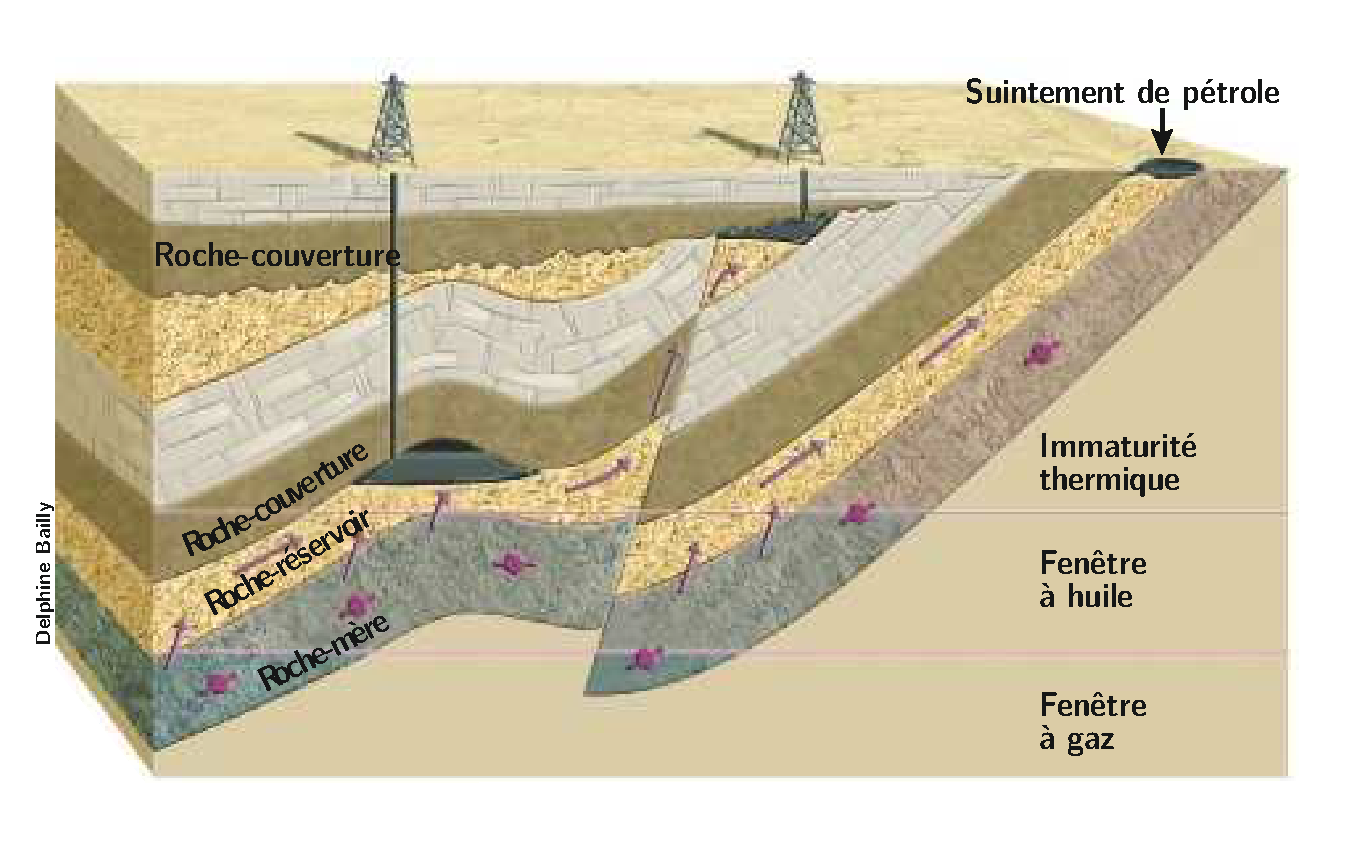
\includegraphics[width=0.8\textwidth]{petrole-profondeur-fig-1}}
	\end{center}
	\textbf{Figure 1.} Un système pétrolier nécessite la présence simultanée de plusieurs éléments, tels une roche-mère, une roche-réservoir, une
	roche-couverture et des pièges, ainsi que des mécanismes géologiques
	nécessaires à la formation et à l’accumulation du pétrole et du gaz
	dans les gisements. Dans les couches profondes, se forme plutôt du
	gaz ; au-dessus, du pétrole ; enfin, dans les couches supérieures, la
	température et le temps de maturation n’ont pas été suffisants pour
	que des hydrocarbures se forment.
\end{tcolorbox}

\textbf{Les systèmes pétroliers}\\

Les bassins sédimentaires sont des dépressions de la croûte terrestre, qui en forme le socle ; ces bassins sont généralement occupés par une mer ou par un océan. Ils résultent de phénomènes géodynamiques associés aux déplacements des plaques de la lithosphère. La croûte terrestre est constituée de roches cristallines d'origine magmatique : granite pour la croûte continentale et basalte pour la croûte océanique. Au cours des temps géologiques, les bassins se remplissent de roches sédimentaires, tels les argiles, les grès (sables consolidés), les carbonates (calcaires) ou les évaporites (sels massifs). Le remplissage dure généralement plusieurs dizaines de millions d'années, à raison de quelques millimètres par an, en moyenne. Le poids des sédiments accumulés participe à la déformation de la croûte terrestre sous-jacente, effet qui s'ajoute aux déformations dues à la tectonique des plaques. La dépression s'accentue, ce qui conduit à des dépôts de sédiments atteignant souvent plusieurs kilomètres. On nomme subsidence cet approfondissement des bassins sous le double effet de la tectonique et de la surcharge sédimentaire ; il atteint 20 kilomètres dans les cas extrêmes. Ainsi, le Bassin parisien est un exemple de bassin sédimentaire reposant sur un socle qui affleure aujourd'hui dans le Massif armoricain, les Vosges et le Massif central ; le remplissage a une épaisseur de 3 000 mètres dans sa partie la plus profonde. C'est au sein des bassins sédimentaires que les hydrocarbures se forment et sont piégés.\\

Premier constituant, la roche-mère est une roche sédimentaire, où une quantité importante de débris organiques s'est accumulée en même temps que le sédiment minéral. Cette matière organique provient de l'accumulation de restes plus ou moins bien conservés de tissus des organismes qui vivaient à proximité. Pour l'essentiel, il s'agit d'algues planctoniques, de plantes supérieures et de bactéries. Pour qu'une roche soit qualifiée de roche-mère, il faut que la matière organique qu'elle contient représente au moins un à deux pour cent du poids de la roche. Ce type de sédiments riches en matière organique est rare, car il requiert des conditions particulières de formation, notamment un écosystème produisant une importante biomasse dont les restes, ayant échappé à la décomposition, sont incorporés dans le sédiment qui se dépose.\\

\textbf{Les roches-mères}\\

Le transport du lieu de production biologique jusqu'au site de dépôt doit être bref et le milieu de sédimentation dépourvu d'oxygène (milieu anoxique). Sinon, les bactéries aérobies et les organismes benthiques prolifèrent et consomment la matière biologique produite. Les roches riches en matière organique sont le plus souvent des roches argileuses ou marneuses (mélange d'argiles et de calcaire). Elles sont de faible granulométrie et, de ce fait, peu poreuses et peu perméables. Élément essentiel d'un système pétrolier, la roche-mère est une « usine à pétrole et à gaz ». Un bassin dépourvu de sédiments riches en matière organique ne peut contenir de champs de pétrole. Toutes les roches-mères ne sont pas équivalentes, mais diffèrent notamment par leur teneur en matière organique, leur volume ou encore la nature du matériau organique fossilisé qu'elles contiennent.\\

On les classe en trois grandes catégories. Le type i est principalement formé de restes de membranes bactériennes et d'algues unicellulaires vivant dans les lacs. Peu répandu, il est d'excellente qualité puisque 70 à 80 pour cent du poids de la matière organique préservée dans le sédiment peuvent se transformer en hydrocarbures, quand les conditions sont favorables. Les roches-mères de type i sont, par exemple, présentes dans les sédiments lacustres des marges occidentales africaines et des marges orientales Sud-américaines (du début du Crétacé), ou sont associées à plusieurs bassins du Tertiaire du Sud-Est asiatique ou à certains bassins continentaux chinois.\\

Le type ii, plus commun, est formé de restes d'algues planctoniques marines. Les roches-mères de la mer du Nord, du Venezuela et d'Arabie saoudite en sont des exemples. Jusqu'à 40 à 60 pour cent du poids de matériel organique qu'elles contiennent se transforment en hydrocarbures dans les conditions optimales. Enfin, le type iii, dont une forme particulière est le charbon, provient des restes de végétaux supérieurs terrestres. Il est, par exemple, caractéristique des roches-mères des deltas fossiles. Le potentiel pétrolier de cette matière organique est relativement faible puisque 10 à 30 pour cent seulement du poids de leur contenu organique peuvent se transformer en hydrocarbures. En revanche, comme les empilements de sédiments qui la contiennent sont souvent épais de plusieurs centaines de mètres, voire de plusieurs kilomètres, la quantité de pétrole produite est importante.\\

Le deuxième constituant d'un système pétrolier est un ensemble de drains généralement constitués de roches poreuses et perméables, ainsi que de fractures et de failles permettant le déplacement des hydrocarbures au sein du bassin sédimentaire. Les roches poreuses et fracturées peuvent également jouer le rôle de roches-réservoirs, où s'accumulent des hydrocarbures. La porosité des roches-réservoirs varie de quelque 5 à 30 pour cent du volume de la roche. Le pétrole et le gaz formés dans la roche-mère sont expulsés vers les drains et s'y déplacent, car leur densité est inférieure à celle de l'eau qui imprègne la totalité des roches sédimentaires : la poussée d'Archimède, qui fait flotter le pétrole sur l'eau, fait migrer les hydrocarbures vers la surface.\\

Troisième constituant, la roche-couverture se situant au-dessus des drains. De par son imperméabilité, elle confine les hydrocarbures dans le système poreux, où ils se déplacent. Il s'agit par exemple de roches argileuses ou de sel massif. L'absence de roche-couverture se traduit par une dispersion des hydrocarbures dans le bassin sédimentaire et par leur fuite vers la surface. Quand ils atteignent le sol, les hydrocarbures y sont détruits par des mécanismes chimiques ou biologiques, comme ceux à l'œuvre lors des pollutions pétrolières accidentelles. On estime que ces suintements naturels d'hydrocarbures dans l'environnement représentent en volume l'équivalent des rejets d'hydrocarbures d'origine humaine.\\

Quatrième constituant d'un système pétrolier, le piège est un obstacle géologique qui arrête la progression des hydrocarbures au cours de leur cheminement vers la surface. Deux sortes de pièges existent : les pièges structuraux sont des accidents géométriques particuliers où le pétrole s'accumule, tels certains plis anticlinaux ou des failles plaçant des barrières imperméables sur le chemin des fluides ; les pièges stratigraphiques résultent de variations locales de la porosité et de la perméabilité de la roche-réservoir. Il peut s'agir, par exemple, du passage d'une roche perméable à une roche imperméable ou de la présence d'une cimentation minérale obstruant les pores de la roche. Les fluides pétroliers – huile ou gaz – s'accumulent dans de tels pièges.\\

Pour qu'un bassin sédimentaire doté de roches-mères, de réservoirs et d'une roche-couverture et contenant des pièges produise du pétrole, il faut aussi qu'il ait eu une histoire thermique adéquate. Celle-ci se déroule alors que la roche-mère est progressivement enfouie au cours des dizaines de millions d'années de remplissage du bassin sédimentaire, associé à la subsidence. Comme la température augmente d'environ 30 °C par kilomètre de profondeur, la chaleur des profondeurs provoque le craquage de la matière organique fossilisée au sein de la roche, c'est-à-dire sa transformation progressive en espèces chimiques de poids moléculaires de plus en plus petits. Le mélange de ces espèces constitue le pétrole, qui sera transformé en un gaz si, la température augmentant encore, le craquage se poursuit. Selon les conditions, on obtient des huiles (c'est la fenêtre à huile) ou du gaz (c'est la fenêtre à gaz). Le craquage est un phénomène cinétique, ce qui signifie que le temps joue un rôle essentiel. Une durée assez longue de craquage peut compenser une température trop faible. Ainsi, si la roche-mère tertiaire qui est à l'origine du pétrole de Californie a atteint sa fenêtre à huile (à 135 °C) au bout de 20 millions d'années, il aura fallu 100 millions d'années à la roche-mère du Bassin parisien pour qu'elle parvienne à 100 °C, c'est-à-dire dans sa propre fenêtre à huile.\\

Les hydrocarbures sont expulsés de la roche-mère : c'est la migration primaire. Cette expulsion se produit vers des drains situés au-dessus ou au-dessous de la roche-mère. Le déplacement des huiles (ou du gaz) résulte de la différence de pression entre les drains et la roche-mère, plus compressible. Après leur expulsion des roches-mères, les hydrocarbures se déplacent vers la surface du bassin le long des drains : c'est la migration secondaire. Leur progression se poursuit jusqu'à ce qu'ils s'accumulent dans un piège.\\

Appliquons ces concepts généraux à la description des provinces pétrolières de l'Atlantique Sud. La formation de cet océan a commencé il y a 140 millions d'années, au début du Crétacé. L'immense masse continentale, la Pangée, s'est scindée en deux continents qui donneront l'Amérique et l'Afrique. Cette séparation a été amorcée par l'amincissement de la croûte terrestre dû à la remontée de roches magmatiques en fusion. Il fut suivi par la phase de rift, c'est-à-dire la rupture de la croûte continentale. À ce stade, l'Atlantique Sud ressemblait à une succession de fossés d'effondrement grossièrement alignés et occupés par de grands lacs. D'épaisses couches sédimentaires riches en matière organique de type i se déposèrent dans ces lacs, s'intercalant avec des sédiments sableux et carbonatés ayant les caractéristiques d'une roche-réservoir.\\

\begin{tcolorbox}[colback=white]
	\begin{center}
		\makebox[\textwidth]{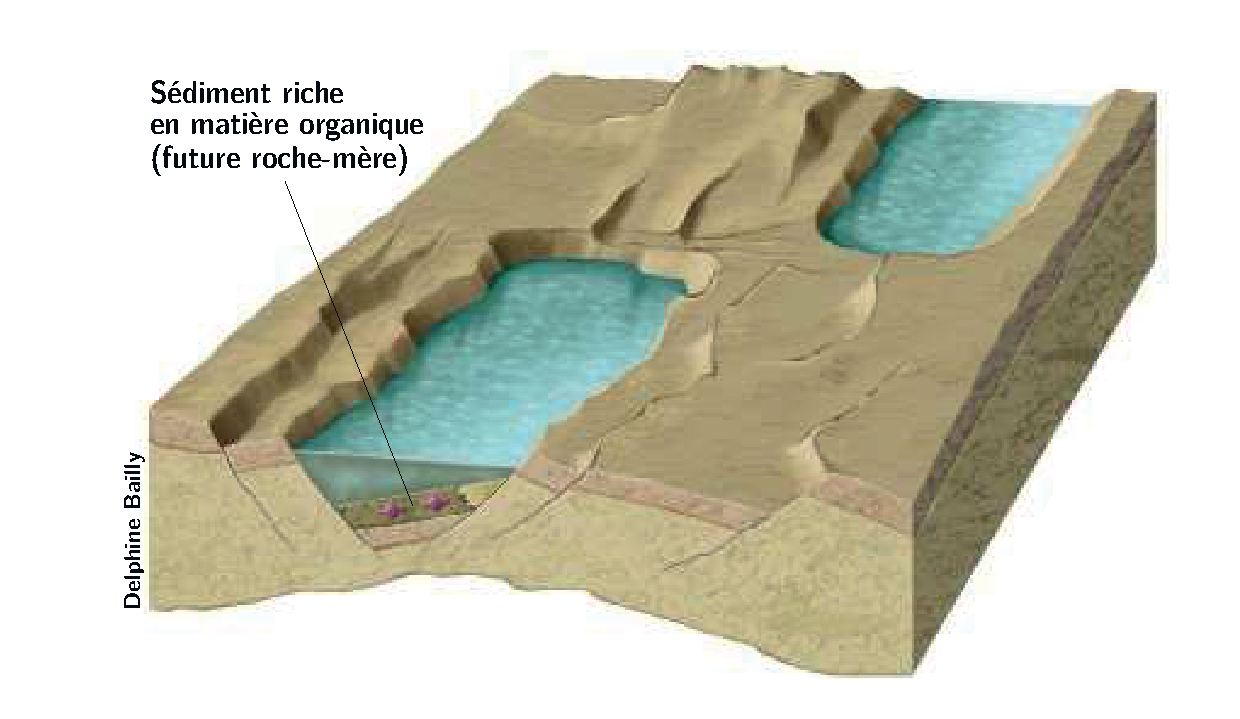
\includegraphics[width=0.8\textwidth]{petrole-profondeur-fig-2}}
	\end{center}
	\textbf{Figure 2.} La phase de « rift » se caractérise par l’établissement d’un
	couloir long de plusieurs milliers de kilomètres où se succèdent des
	fossés d’effondrement occupés par de grands lacs. C’est dans ces lacs
	que se sont déposées d’épaisses couches sédimentaires riches en matière
	organique de type I, s’intercalant avec des sédiments sableux et carbonatés qui peuvent présenter les propriétés d’une roche-réservoir.
	
\end{tcolorbox}

\textbf{La formation de l'Atlantique Sud}\\

Cette phase fut suivie d'une phase d'ouverture : en s'écartant, les domaines continentaux formèrent un bassin sédimentaire de plus en plus large. Au cours de cette dérive, les continents africain et américain entraînèrent avec eux, en les conservant sur leurs marges respectives, les restes des bassins lacustres du rift. Les roches-mères les plus riches en pétrole de l'Atlantique Sud sont situées dans ces restes de bassins lacustres, à l'origine d'une grande partie des réserves pétrolières de l'Angola, du Congo, du Gabon et du Brésil. En s'éloignant, les deux continents ont ensuite permis aux eaux marines venant de l'océan de s'engouffrer périodiquement, dans les bassins en formation. Le remplissage épisodique de ces bassins par de l'eau de mer alternait avec des périodes d'isolement de l'océan au cours desquelles les eaux marines piégées s'évaporaient donnant alors naissance à d'épaisses couches de sels. Datées d'environ 120 millions d'années, celles-ci recouvrirent les bassins lacustres et ont donné les couches salifères de l'Atlantique Sud.\\

L'ouverture de l'Atlantique Sud se poursuivant, la jeune dorsale médio-océanique commença à émettre des roches volcaniques basaltiques à l'origine de la croûte océanique. Progressivement, le régime marin s'installa. Le dépôt épisodique de couches de sel fut remplacé par une sédimentation calcaire et marneuse, mais aussi gréseuse, produisant d'excellentes roches-réservoirs. Cependant, ce nouvel océan était encore peu accessible aux eaux marines et restait confiné. Cette situation propice à l'établissement de conditions anoxiques permit le dépôt intermittent de nouvelles roches-mères, de type ii. Elle s'acheva il y a quelque 80 millions d'années. Le bassin océanique était devenu trop large pour conserver des conditions anoxiques : des eaux marines contenant de l'oxygène dissous commencèrent à affluer. Les conditions de préservation des roches-mères n'étaient plus assurées.\\

Il faudra attendre la fin du Crétacé, mais surtout le début du Tertiaire, il y a environ 50 millions d'années, pour que des conditions propices à la mise en place de nouveaux systèmes pétroliers réapparaissent. Ce fut le cas après une accumulation suffisante de sédiments arrachés aux continents dans les exutoires de bassins versants, face aux deltas notamment. Ce régime de dépôt a été favorisé par le refroidissement de la croûte océanique la plus ancienne, située au niveau des marges continentales. Ce refroidissement rend la croûte plus dense et, par conséquent, plus lourde. Elle s'enfonce par un mécanisme que les géologues nomment flexuration. Le phénomène crée un espace disponible pour l'accumulation de grandes quantités de sédiments issus du continent. L'entassement de quantités importantes de sédiments provoque l'enfouissement et la maturation thermique des roches-mères. D'épaisses séries sédimentaires argilo-sableuses s'accumulèrent par exemple dans le delta du Niger. C'est dans ces complexes sédimentaires détritiques que l'on trouve par endroits des niveaux riches en matière organique de type iii, contenant des débris de végétaux continentaux. Les hydrocarbures sont confinés dans des chenaux sableux, restes des couloirs sous-marins de transport des sédiments vers les grandes profondeurs. Ces réservoirs sont noyés au sein d'argiles jouant le rôle de couverture.\\

\begin{tcolorbox}[colback=white]
	\begin{center}
		\makebox[\textwidth]{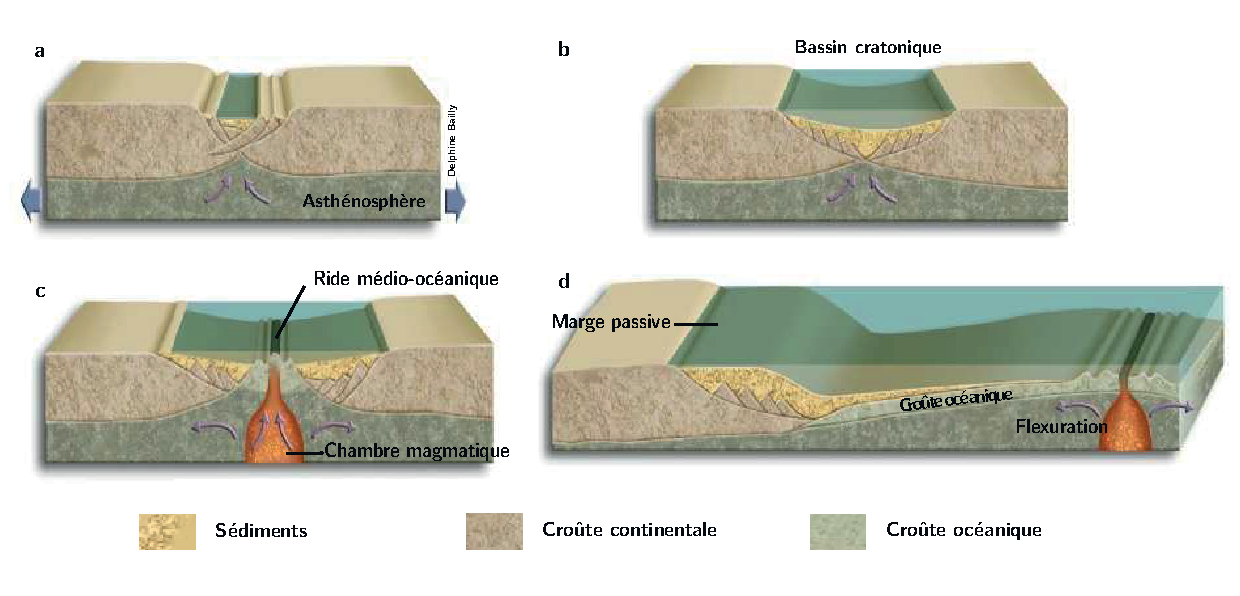
\includegraphics[width=\textwidth]{petrole-profondeur-fig-3}}
	\end{center}
	\textbf{Figure 3.} L’ouverture a commencé par la rupture (phase de Rift, a) de la masse continentale initiale, la Pangée, provoquée par un phénomène régional
	de remontée magmatique le long de la future ride médio-océanique.
	La croûte continentale s’est rompue par endroits, et les fossés d’effondrement qui en ont résulté ont été occupés par de grands lacs. Le couloir initial s’est progressivement élargi en donnant naissance à un bassin
	marin, le bassin cratonique (b), dont le plancher était constitué de croûte
	continentale. Le magma issu de l’asthénosphère a alors commencé à
	être émis au niveau de la ride médio-océanique, formant une croûte océanique basaltique qui constituera le plancher de l’océan : c’était la phase
	de drift (c). L’ouverture océanique se poursuivant, les parties les plus
	anciennes de cette croûte océanique, c’est-à-dire celles qui sont les plus
	proches des marges continentales, se sont progressivement refroidies,
	leur densité a augmenté, de sorte qu’elles sont devenues plus lourdes.
	Elles se sont gauchies sous l’effet de leur poids : c’est le phénomène de
	flexuration (d). Dans les creux ainsi ménagés, les sédiments arrachés
	à la terre se sont accumulés dès la fin du Crétacé, et surtout au Tertiaire, il y a environ 50 millions d’années. Les conditions étaient alors
	réunies pour que du gaz et du pétrole s’accumulent par endroits.
\end{tcolorbox}

\newpage
Cette histoire géologique est à l'origine d'une grande richesse pétrolière. Plusieurs traits de la région expliquent pourquoi. Tout d'abord, la région contient plusieurs familles de roches-mères d'âges géologiques différents. Cette situation a produit un grand nombre de systèmes pétroliers comparables de part et d'autre de l'Atlantique. Ainsi, le bassin de Campos au large du Brésil et celui du bas Congo contiennent tous deux des roches-mères lacustres (type i) déposées au début de la formation de l'Atlantique et des roches-mère marines (type ii) plus récentes datant du Crétacé moyen (100 millions d'années). Toutefois, tandis que les roches-mères congolaises de types i et ii ont produit des hydrocarbures, seules les roches lacustres de type i ont atteint la fenêtre à huile du côté brésilien.\\

D'où vient cette dissymétrie ? Pour l'essentiel, elle résulte du rehaussement du socle africain dû à la collision des plaques africaine et européenne. Accroissant l'érosion de l'Afrique, cette élévation des masses continentales a mobilisé de grandes quantités d'alluvions fluviales, qui se sont déposées dans les deltas durant le Tertiaire (entre 65 et 2 millions d'années) pour atteindre parfois 11 kilomètres d'épaisseur, comme c'est le cas dans l'embouchure du Niger. Ceci explique que beaucoup de roches-mères africaines de type ii déposées après les niveaux de sel aient produit des hydrocarbures, alors que du côté brésilien, seules les roches-mères lacustres de type i déposées avant l'épisode salifère ont atteint la fenêtre à huile.\\

\textbf{La richesse pétrolière de l'Atlantique Sud}\\

Outre cette sédimentation importante, les marges de l'Atlantique Sud comptent un grand nombre de failles. Ces dernières forment les drains efficaces par lesquels les hydrocarbures migrent des roches-mères vers des réservoirs supérieurs. Elles ont été formées lors de la phase d'ouverture, ou par des glissements de blocs de sédiments au cours des phases ultérieures. Elles sont souvent associées à la présence de couches de sel déposées après les épisodes de sédimentation lacustre. Le sel crée des surfaces de décollement sur lesquelles les sédiments inclinés par la flexuration glissent facilement. Caractéristique supplémentaire, les marges de l'Atlantique Sud contiennent d'excellentes roches-réservoirs réparties dans l'ensemble de la pile sédimentaire. De telles roches sont fréquentes dans les sédiments présalifères, dans les calcaires postsalifères et dans les réservoirs sableux du Tertiaire. Ces derniers sont constitués de chenaux et de lobes sableux déposés le long de la pente et au pied du talus continental par le transport en masse de sédiments. Il y a quelques années encore, on ignorait leur répartition, leur architecture et leur structure interne. Dans certains cas, ces réservoirs sont peu enfouis et mal consolidés, ce qui est source de difficultés techniques au cours de l'exploitation du champ de pétrole (il existe, par exemple, des risques d'affaissements). Par ailleurs, les couvertures associées à ces réservoirs sont parfois peu compactes et laissent les hydrocarbures s'échapper.\\

Le sous-sol de l'Atlantique contient aussi de bonnes roches-couverture, soit argileuses, soit salifères. Près du rivage, la couche de sel est continue. En revanche, loin du rivage, elle est morcelée. De plus en plus discontinue à mesure que l'on s'éloigne du continent, la couche salifère finit par former des « radeaux », isolés les uns des autres. Cet agencement des couches salifères se traduit par le confinement des huiles sous le sel et, en l'absence de sel, par le passage des huiles vers des réservoirs supérieurs. Ainsi, la géométrie des terrains sédimentaires des marges de l'Atlantique Sud a multiplié les pièges : des radeaux de sel, de grands plis anticlinaux calcaires du Crétacé et de grandes ondulations au sein des sédiments du Tertiaire contenant des chenaux englobés dans des argiles imperméables, par exemple.\\

Pendant les 140 millions d'années d'histoire géologique de l'Atlantique, de nombreux systèmes pétroliers se sont formés, puis leurs réservoirs se sont emplis d'huiles et de gaz. Certains se sont formés au-delà de 2 000 mètres de profondeur d'eau. Longtemps, ces gisements sont restés hors de portée, mais ces dix dernières années, plusieurs grandes compagnies pétrolières ont appris à travailler au-delà de 500 mètres de profondeur, et parfois jusqu'à des milliers de mètres sous la surface de l'océan. Jusqu'à quel point peut-on étendre le cadre géologique des domaines profonds aux zones ultraprofondes ? Aujourd'hui, les géologues disposent de concepts et de méthodes leur permettant de relever le défi de l'exploration du domaine profond. Ils savent comment se forme un système pétrolier, et parviennent à visualiser sa structure et son contenu à l'aide de la sismique réflexion, sorte d'échographie appliquée aux terrains géologiques. Pour mettre en œuvre cette méthode, on crée des ondes à la surface de la mer, par exemple à l'aide de canons à air, puis on utilise les ondes réfléchies sur les différentes structures géologiques contenues dans la pile sédimentaire pour créer des images.\\

\textbf{Les incertitudes liées à l'exploration de l'ultraprofond}\\

Ces images du sous-sol sont à deux, voire, de plus en plus souvent, à trois dimensions, comme celles que l'on produit pour explorer l'offshore profond. Elles doivent être calibrées à l'aide de toutes les informations disponibles sur la zone concernée, notamment celles qui proviennent des forages existants. Nombre d'explorateurs pétroliers s'appuient aussi sur des simulations numériques de systèmes pétroliers. Grâce à ces simulateurs, on reconstitue notamment l'histoire du remplissage d'un bassin au cours des temps géologiques. On reproduit aussi l'histoire thermique des sédiments, en particulier celle de la roche-mère, la formation des hydrocarbures, leur migration au sein du bassin, puis leur accumulation dans les pièges. Dans le meilleur des cas, les simulateurs livrent même la nature des hydrocarbures retenus dans les gisements (par exemple huile ou gaz). Même si quelques incertitudes demeurent, quant à la précision des images et des résultats des simulations, la méthode réduit notablement le risque d'échec d'un forage.\\

Jusqu'où peut-on trouver des roches-mères et des réservoirs potentiels ? Pour le moment nous l'ignorons. Une deuxième incertitude est liée à la variation de l'épaisseur des sédiments. Cette épaisseur croît jusque dans le domaine profond, sur la marge continentale, mais diminue ensuite inéluctablement quand on s'éloigne vers le large. Moins enfouies, les roches-mères sont moins matures à âge égal. Les roches-mères lacustres qui se trouvent dans la fenêtre à gaz, dans le domaine profond, sont, si elles existent, plus probablement dans la fenêtre à huile dans le domaine ultraprofond.\\

De même, les roches-mères crétacées marines qui se trouvaient dans la fenêtre à huile dans le domaine profond peuvent même être immatures dans le domaine ultraprofond. L'impact de l'enfouissement est d'autant plus important que le flux thermique dont bénéficient les sédiments diminue vers le large : la croûte continentale contenant des isotopes radioactifs sources de chaleur s'amincit, puis est remplacée par une croûte océanique pauvre en éléments radioactifs. Le refroidissement de la croûte et la diminution de l'épaisseur sédimentaire se conjuguent pour imposer une limite extrême, au-delà de laquelle aucun système pétrolier ne peut produire d'hydrocarbures. Les simulations nous donneront cette limite ultime dès que nous aurons rassemblé suffisamment de données provenant du domaine ultraprofond et que nous les aurons calibrées.\\

Les zones de bassins sédimentaires situées à très grande profondeur sont souvent d'une grande complexité géologique. Leurs structures tourmentées résultent de la tectonique compressive liée aux mouvements gravitaires qu'elles ont subis. Ceci se traduit par des chevauchements de compartiments sédimentaires. L'inclinaison importante des blocs sédimentaires et la présence de sel compliquent l'interprétation des images sismiques du sous-sol. Enfin, il est possible que les gisements ultraprofonds soient peu enfouis. Or, dans les systèmes pétroliers peu enfouis, la température n'est pas trop élevée, ce qui permet à la vie bactérienne de se maintenir (elle ne disparaît qu'au-dessus de 90 °C). Les pétroles de certains de ces gisements subissent une biodégradation qui les transforme en « huile lourde », un liquide dense et visqueux peu recherché et difficile à extraire.\\

Ces difficultés et ces risques sont considérables. Toutefois, dans les années 1970, les obstacles techniques et scientifiques à l'exploration et à l'exploitation des gisements du domaine profond semblaient insurmontables. Pourtant, certains se sont lancés, et la production est déjà importante. Nous trouvons-nous, aujourd'hui, vis-à-vis du domaine ultraprofond dans la situation où nous nous trouvions face au domaine profond dans les années 1970 ? Il nous faudra quelques années de patience pour avoir la réponse.


\begin{tcolorbox}[colback=white]
	\begin{center}
		\makebox[\textwidth]{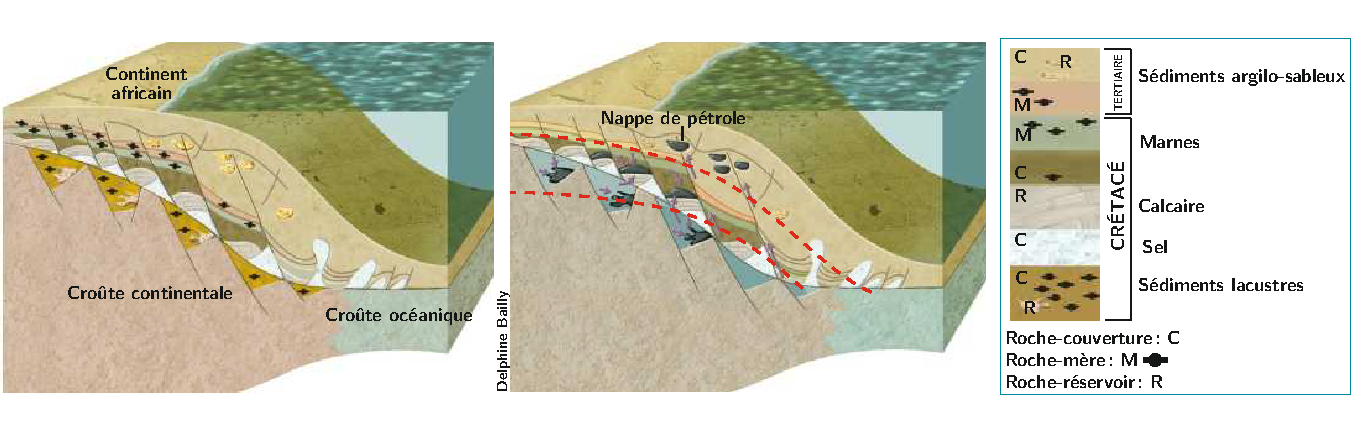
\includegraphics[width=\textwidth]{petrole-profondeur-fig-4}}
	\end{center}
	\textbf{Figure 4.} Coupe géologique schématique d’une marge de l’Atlantique Sud, au large du Gabon,
	du Congo et de l’Angola. Les échelles n’ont pas été respectées en ce qui concerne l’épaisseur des croûtes continentale et océanique, qui mesurent respectivement entre 5 et 15 kilomètres, et entre 30 et 65 kilomètres. On a schématisé le sous-sol de la côte jusqu’à une centaine de kilomètres au large. L’épaisseur de la pile sédimentaire représente ici jusqu’à
	une dizaine de kilomètres. Des sédiments lacustres, contenant des roches-mères de type I sont confinés dans des dépressions de la croûte continentale (à gauche). Ils sont surmontés de dépôts de sel, de roches calcaires (qui constituent souvent de très bons réservoirs),puis de marnes, dont certaines sont des roches-mères de type II. Au-dessus, les couches argilo-sableuses contiennent des roches-mères de type III et des réservoirs localisés dans
	des chenaux et dans des lobes sableux. Des hydrocarbures se sont formés dans les différentes roches-mères quand les conditions thermiques étaient adéquates. L’expulsion des
	roches-mères et la migration secondaire le long des drains acheminent (à droite, les flèches) les hydrocarbures (pétrole et gaz) vers des pièges où ils restent confinés par la
	roche-couverture imperméable. Dans la fenêtre à huile (entre les deux lignes en pointillés
	rouges), les hydrocarbures formés sont du pétrole. La fenêtre à gaz est située juste sous la fenêtre à huile (au-dessous de la ligne en pointillés inférieure).
	
\end{tcolorbox}

\end{document}


